\documentclass{scrreprt}
\usepackage{listings}
\usepackage{underscore}
\usepackage{graphicx}
\usepackage[bookmarks=true]{hyperref}
\usepackage[utf8]{inputenc}

\usepackage[table]{xcolor}
\usepackage{float}
\usepackage{pifont}
\usepackage{amssymb}
\usepackage[inline]{enumitem}
\usepackage{adjustbox}

\hypersetup{
	pdftitle={Software Requirement Specification},    % title
	pdfauthor={Jean-Philippe Eisenbarth},                     % author
	pdfsubject={TeX and LaTeX},                        % subject of the document
	pdfkeywords={TeX, LaTeX, graphics, images}, % list of keywords
	colorlinks=true,       % false: boxed links; true: colored links
	linkcolor=blue,       % color of internal links
	citecolor=black,       % color of links to bibliography
	filecolor=black,        % color of file links
	urlcolor=purple,        % color of external links
	linktoc=page            % only page is linked
}%
\def\myversion{2.0 }
\date{}
%\title
\usepackage{hyperref}
\begin{document}
	
	\begin{flushright}
		\rule{10cm}{5pt}\vskip1cm
		\begin{bfseries}
			\Huge{DOCUMENTO DE REQUISITOS\\ESPECIFICAÇÃO}\\
			\vspace{1.5cm}
			PARA\\
			\vspace{1.5cm}
			DASHBOARD\\ SMART OVITRAPS\\
			\vspace{1.5cm}
			\LARGE{Version \myversion}\\
			\vspace{1.5cm}
			Preparado por : Daniel Pinheiro dos Reis\\
			\vspace{1.5cm}
			\today\\
		\end{bfseries}
	\end{flushright}
		
	\chapter{Introdução}
	
	\section{Proposta}
	SMART OVITRAP é uma plataforma integrada com armadilhas ovitraps para monitoramento e controle de arbovírus como dengue, zika e chikungunya. 
	
	\section{Público Alvo}
	Prefeituras, órgãos governamentais, grandes empresas ou entusiastas interessados no combate e monitoramento de arbovírus.
	\section{Escopo de projeto}
	SMART OVITRAP cria um espaço para que gestores e agentes de órgãos de saúde ou saneamento ou grandes empresas possam fazer o controle e monitoramento das armadilha ovitraps instaladas na sua região.
	\newline
	O sistema consiste de uma plataforma com 3 tipos de usuários Agentes, Gestores e Administradores .
	Para uma empresa ou prefeitura utilizar a plataforma é preciso previamente solicitar o cadastro para os Administradores do Sistema. Depois de cadastrado a empresa ou prefeitura e um primeiro usuário gestor, o gestor, poderá logar na plataforma com sua senha e se desejar cadastrar novos gestores ou novos agentes para sua prefeitura ou empresa. 
	
	\newpage
	\chapter{Descrição Geral}
	
	\section{Perspectiva do Produto}
	SMART OVITRAP substitui as armadilhas ovitraps convencionais, permitindo o monitoramento das mesmas de maneira remota, o único trabalho de campo necessário é a troca da água ou da fita adesiva, o calendário de manutenções e a contagem de mosquito são acessados de maneira remota através de qualquer navegador de internet.
	
	\section{Casos de Uso e Características do Sistema}
	SMART OVITRAP possui três tipos de usuários:
	
	\begin{itemize}
		\item Administradores do Sistema
		\item Gestores
		\item Agentes
	\end{itemize}
	
	SMART OVITRAP possui uma plataforma única com funcionalidades diferentes para cada tipo de usuário.
	
	Gestore
	
	\begin{figure}[H]
		\centering
		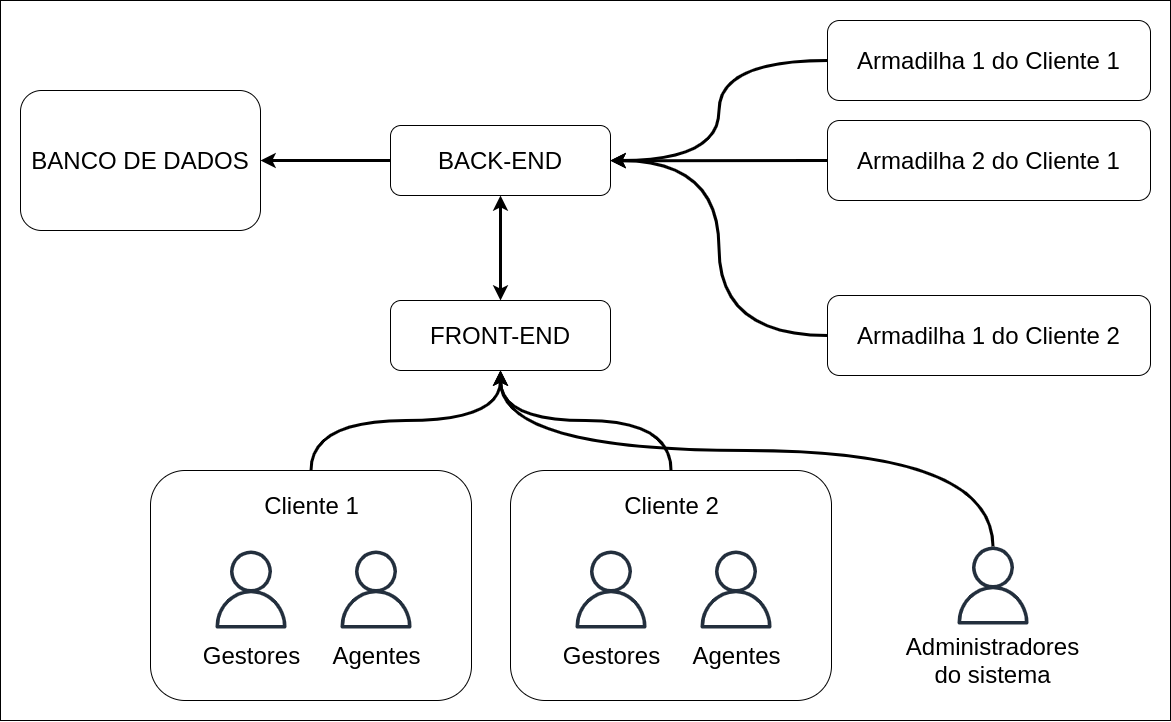
\includegraphics[scale=0.3]{DiagramaPlataforma.png}
		\caption{Diagrama do sistema}
	\end{figure}
		
	Administradores do Sistema têm permissões de cadastrar: empresas, gestores e agentes.
	Gestores podem cadastrar: gestores, agentes e armadilhas. Agentes conseguem visualizar todas as armadilhas porém só podem editar e excluir as que foram cadastradas por eles.
	
	Os Administradores de Sistema podem: 
	\begin{itemize}
		\item  Cadastrar, listar, alterar e deletar empresas ou prefeituras do sistema. 
		\item  Cadastrar, listar alterar e deletar usuários de determinada empresa ou prefeitura 
		\item  Cadastrar, listar alterar e deletar armadilhas de determinada empresa ou prefeitura
	\end{itemize}
	
	Os Gestores podem:
	\begin{itemize}
		\item  Cadastrar, listar, alterar e deletar Gestores da sua empresa
		\item  Cadastrar, lista, alterar e deletar Agentes da sua empresa
		\item  Cadastrar, listar, alterar e deletar Armadilhas da sua empresa
	\end{itemize}
	
	Os Agentes podem:
	\begin{itemize}
		\item Cadastrar e listar suas próprias armadilhas
		\item Visualizar o total de capturas de cada armadilha da sua empresa
	\end{itemize}
	
	\begin{figure}[H]
		\centering
		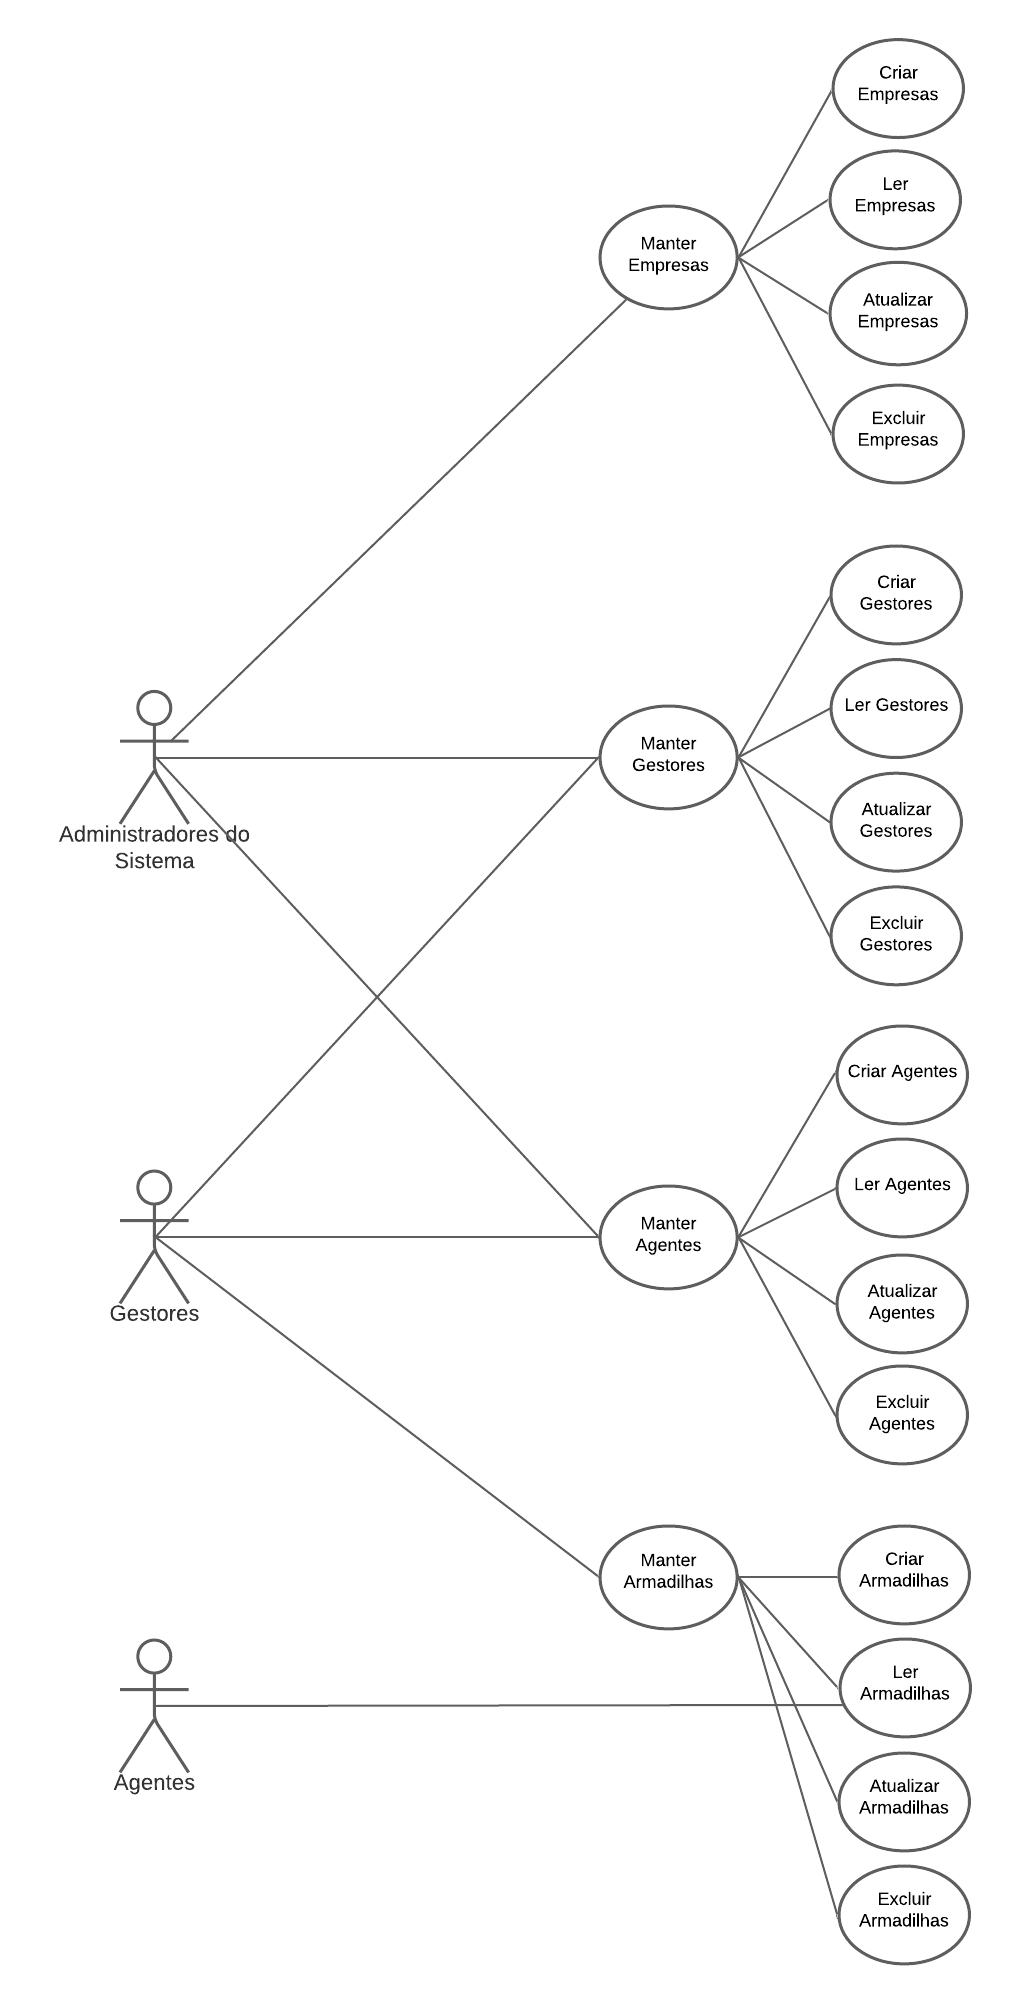
\includegraphics[width=8cm]{casosDeUso.png}
		\caption{Diagrama de Casos de Uso}
	\end{figure}
	
	\section{Funções do Produto}
	Permitir o monitoramento remoto de armadilhas ovitraps, quanto a quantidade de mosquitos, a localização da armadilha, a ultima manutenção realizada e outros dados que forem necessários para geração de relatórios e tomada de decisão de organizações interessadas no combate aos arbovírus 
	
	\section{Ambiente de Operação}
	A plataforma de monitoramento pode ser acessada de qualquer dispositivo conectado a internet e que possua um navegador de internet.
	
	\section{Design}
	O design da plataforma seguirá as 10 heurísticas de Nielsen para garantir os padrões de usabilidade. O desenvolvimento da plataforma seguirá rigorosamente este documento, os requisitos e a modelagem das telas aqui explicitados
	
	\chapter{Funcionalidades do Sistema}
	Esta seção descreve todos os requisitos e funcionalidades do sistema e as convenções e termos utilizados.
	
	\section{Descrição e Prioridade}
	Esta seção descreve os usuários e requisitos da plataforma: 
	
	Os usuários são divididos em 3 grupos:  
	
	\begin{itemize}
		\item Administradores do Sistema
		\item Gestores
		\item Agentes
	\end{itemize}
	
	Os requisitos de cada plataforma são divididos em dois grupos descritos abaixo:
	
	\begin{itemize}
		\item Requisito funcional (RF): Requisitos de extrema importância para o funcionamento da plataforma, estão diretamente ligados  às funcionalidades do sistema.
		\item Requisito não-funcional (RNF): Requisitos ligado às métricas e atributos de qualidade do sistema.
	\end{itemize}
	
	Cada um dos requisitos acima possui uma das três prioridades abaixo:
	
	\begin{itemize}
		\item Essencial: Requisitos imprescindíveis para o funcionamento correto do sistema.
		\item Importante: Requisitos não essenciais para o funcionamento do sistema, mas que sem eles o sistema não se comporta de maneira satisfatória. 
		\item Desejável: Requisitos que não interferem no funcionamento do sistema, complementos que auxiliam no funcionamento do sistema.
	\end{itemize}
	
	
	\subsection{Requisitos Funcionais}
	% REQUISITO START %
	\begin{center}
		\noindent\rule{16cm}{0.4pt}
		\textbf{[RF01] Logar na plataforma}
		\noindent\rule{16cm}{0.4pt}
	\end{center}
	\textbf{Usuário:} Administradores do Sistema, Gestores e Agentes
	
	O sistema deve permitir o login na plataforma.
	
	\begin{center}
		\begin{adjustbox}{width=\textwidth}      \begin{tabular}{ |c|c|c|c|c| } 
			\hline
			\rowcolor{lightgray} Campo & Descrição & Tamanho & Métrica & Obrigatório \\
			\hline
			E-mail & E-mail do usuário  & 255 & caracteres & sim \\ 
			\hline
			Senha & Senha do usuário & 64 & caracteres & sim \\
			\hline
		\end{tabular}    \end{adjustbox}
	\end{center}
	
	\textbf{Prioridade: }\begin{itemize*}
		\item[\hspace{1cm}\rlap{\raisebox{0.2ex}{\hspace{0.4ex}\scriptsize \ding{56}}}$\square$]
		Essencial
		\item[\hspace{1cm}$\square$]
		Importante
		\item[\hspace{1cm}$\square$]
		Desejável
	\end{itemize*}
	% REQUISITO END %
	% REQUISITO START %
	\begin{center}
		\noindent\rule{16cm}{0.4pt}
		\textbf{[RF02] Cadastrar Administradores do Sistema}
		\noindent\rule{16cm}{0.4pt}
	\end{center}
	\textbf{Usuário:} Administradores do Sistema
	
	O sistema deve permitir o cadastro de usuários do tipo Administradores do Sistema
	
	\begin{center}
		\begin{adjustbox}{width=\textwidth}      \begin{tabular}{ |c|c|c|c|c| } 
			\hline
			\rowcolor{lightgray} Campo & Descrição & Tamanho & Métrica & Obrigatório \\
			\hline
			Nome & Nome completo do usuário a ser cadastrado & 255 & caracteres & sim \\ 
			\hline
			E-mail & E-mail do usuário a ser cadastrado & 255 & caracteres & sim \\ 
			\hline
			Perfil & Perfil do usuário a ser cadastrado & 64 & caracteres & sim \\ 
			\hline
			Apelido & Apelido do usuário a ser cadastrado & 64 & caracteres & não \\
			\hline
		\end{tabular}    \end{adjustbox}
	\end{center}
	
	\textbf{Prioridade: }\begin{itemize*}
		\item[\hspace{1cm}\rlap{\raisebox{0.2ex}{\hspace{0.4ex}\scriptsize \ding{56}}}$\square$]
		Essencial
		\item[\hspace{1cm}$\square$]
		Importante
		\item[\hspace{1cm}$\square$]
		Desejável
	\end{itemize*}
	% REQUISITO END %
	% REQUISITO START %
	\begin{center}
		\noindent\rule{16cm}{0.4pt}
		\textbf{[RF03] Cadastrar Empresas (Clientes)}
		\noindent\rule{16cm}{0.4pt}
	\end{center}
	\textbf{Usuário:} Administradores do Sistema
	
	O sistema deve permitir o cadastro de Empresas (Clientes)
	
	\begin{center}
		\begin{adjustbox}{width=\textwidth}      \begin{tabular}{ |c|c|c|c|c| } 
				\hline
				\rowcolor{lightgray} Campo & Descrição & Tamanho & Métrica & Obrigatório \\
				\hline
				Nome & Nome completo da empresa a ser cadastrada & 255 & caracteres & sim \\ 
				\hline
				E-mail & E-mail da empresa a ser cadastrada & 255 & caracteres & sim \\ 
				\hline
				CPF/CNPJ & CPF/CNPJ da empresa a ser cadastrada & 14/18 & caracteres & sim \\ 
				\hline
				PF/PJ & Se o documento é pessoa física ou jurídica & 2 & caracteres & sim \\ 
				\hline
				Site & Site da empresa a ser cadastrada & 255 & caracteres & não \\ 
				\hline
				CEP & CEP da empresa a ser cadastrada & 9 & caracteres & não \\ 
				\hline
				Endereço & Endereço da empresa a ser cadastrada & 255 & caracteres & não \\ 
				\hline
				Número & Número da empresa a ser cadastrada & 16 & caracteres & não \\ 
				\hline
				Bairro & Bairro da empresa a ser cadastrada & 64 & caracteres & não \\ 
				\hline
				Cidade & Cidade da empresa a ser cadastrada & 64 & caracteres & não \\ 
				\hline
				Estado & Estado da empresa a ser cadastrada & 64 & caracteres & não \\ 
				\hline
				Telefone & Telefone da empresa a ser cadastrada & 64 & caracteres & não \\ 
				\hline
				Observações & Observações da empresa a ser cadastrada & 255 & caracteres & não \\
				\hline
		\end{tabular}    \end{adjustbox}
	\end{center}
	
	\textbf{Prioridade: }\begin{itemize*}
		\item[\hspace{1cm}\rlap{\raisebox{0.2ex}{\hspace{0.4ex}\scriptsize \ding{56}}}$\square$]
		Essencial
		\item[\hspace{1cm}$\square$]
		Importante
		\item[\hspace{1cm}$\square$]
		Desejável
	\end{itemize*}
	% REQUISITO END %
	
	% REQUISITO START %
	\begin{center}
		\noindent\rule{16cm}{0.4pt}
		\textbf{[RF04] Cadastrar Usuários}
		\noindent\rule{16cm}{0.4pt}
	\end{center}
	\textbf{Usuário:} Administradores do Sistema, Gestores e Agentes
	
	O sistema deve permitir o cadastro de usuários do tipo administradores do sistema, gestores e agentes, sendo que os administradores do 
	sistema somente podem ser cadastrados por administradores do sistema. Gestores podem cadastrar outros gestores e agentes.
	
	\begin{center}
		\begin{adjustbox}{width=\textwidth}      \begin{tabular}{ |c|c|c|c|c| } 
			\hline
			\rowcolor{lightgray} Campo & Descrição & Tamanho & Métrica & Obrigatório \\
			\hline
			Nome & Nome completo do usuário a ser cadastrado & 255 & caracteres & sim \\ 
			\hline
			E-mail & E-mail do usuário a ser cadastrado & 255 & caracteres & sim \\ 
			\hline
			Perfil & Perfil do usuário a ser cadastrado: Gestor ou Agente & 64 & caracteres & sim \\ 
			\hline
			Apelido & Apelido do usuário a ser cadastrado & 64 & caracteres & não \\
			\hline
		\end{tabular}    \end{adjustbox}
	\end{center}
	
	\textbf{Prioridade: }\begin{itemize*}
		\item[\hspace{1cm}\rlap{\raisebox{0.2ex}{\hspace{0.4ex}\scriptsize \ding{56}}}$\square$]
		Essencial
		\item[\hspace{1cm}$\square$]
		Importante
		\item[\hspace{1cm}$\square$]
		Desejável
	\end{itemize*}
	% REQUISITO END %
	% REQUISITO START %
	\begin{center}
		\noindent\rule{16cm}{0.4pt}
		\textbf{[RF05] Editar Empresa}
		\noindent\rule{16cm}{0.4pt}
	\end{center}
	\textbf{Usuário:} Administradores do Sistema
	
	O sistema deve permitir ao cliente editar os dados da própria empresa
	
	\begin{center}
		\begin{adjustbox}{width=\textwidth}      \begin{tabular}{ |c|c|c|c|c| } 
			\hline
			\rowcolor{lightgray} Campo & Descrição & Tamanho & Métrica & Obrigatório \\   
			\hline
			Site & Site da empresa a ser cadastrada & 255 & caracteres & não \\ 
			\hline
			CEP & CEP da empresa a ser cadastrada & 9 & caracteres & não \\ 
			\hline
			Endereço & Endereço da empresa a ser cadastrada & 255 & caracteres & não \\ 
			\hline
			Número & Número da empresa a ser cadastrada & 16 & caracteres & não \\ 
			\hline
			Bairro & Bairro da empresa a ser cadastrada & 64 & caracteres & não \\ 
			\hline
			Cidade & Cidade da empresa a ser cadastrada & 64 & caracteres & não \\ 
			\hline
			Estado & Estado da empresa a ser cadastrada & 64 & caracteres & não \\ 
			\hline
			Telefone & Telefone da empresa a ser cadastrada & 64 & caracteres & não \\ 
			\hline
			Observações & Observações da empresa a ser cadastrada & 255 & caracteres & não \\    
			\hline
		\end{tabular}    \end{adjustbox}
	\end{center}
	
	\textbf{Prioridade: }\begin{itemize*}
		\item[\hspace{1cm}\rlap{\raisebox{0.2ex}{\hspace{0.4ex}\scriptsize \ding{56}}}$\square$]
		Essencial
		\item[\hspace{1cm}$\square$]
		Importante
		\item[\hspace{1cm}$\square$]
		Desejável
	\end{itemize*}
	% REQUISITO END %
	% REQUISITO START %
	\begin{center}
		\noindent\rule{16cm}{0.4pt}
		\textbf{[RF06] Cadastrar Armadilhas}
		\noindent\rule{16cm}{0.4pt}
	\end{center}
	\textbf{Usuário:} Administradores do Sistema, Gestores e Agentes
	
	O sistema deve permitir o cadastro de armadilhas
	
	\begin{center}
		\begin{adjustbox}{width=\textwidth}      \begin{tabular}{ |c|c|c|c|c| } 
			\hline
			\rowcolor{lightgray} Campo & Descrição & Tamanho & Métrica & Obrigatório \\
			\hline
			Nome & Nome para armadilha Ex: Quintal, Jardim & 255 & caracteres & sim \\ 
			\hline  
			UUID & UUID que deve ser inserido na armadilha & 255 & caracteres & sim \\ 
			\hline  
		\end{tabular}    \end{adjustbox}
	\end{center}
	
	\textbf{Prioridade: }\begin{itemize*}
		\item[\hspace{1cm}\rlap{\raisebox{0.2ex}{\hspace{0.4ex}\scriptsize \ding{56}}}$\square$]
		Essencial
		\item[\hspace{1cm}$\square$]
		Importante
		\item[\hspace{1cm}$\square$]
		Desejável
	\end{itemize*}
	% REQUISITO END %
	% REQUISITO START %
	\begin{center}
		\noindent\rule{16cm}{0.4pt}
		\textbf{[RF07] Obter quantidade de mosquitos da armadilha}
		\noindent\rule{16cm}{0.4pt}
	\end{center}
	\textbf{Usuário:} Administradores do Sistema, Gestores e Agentes
	
	O sistema deve fornecer a quantidade de mosquitos por armadilha
	
	\begin{center}
		\begin{adjustbox}{width=\textwidth}      \begin{tabular}{ |c|c|c|c|c| } 
			\hline
			\rowcolor{lightgray} Campo & Descrição & Tamanho & Métrica & Obrigatório \\
			\hline
			Quantidade & Quantidade de mosquitos & - & inteiro & - \\    
			\hline 
		\end{tabular}    \end{adjustbox}
	\end{center}
	
	\textbf{Prioridade: }\begin{itemize*}
		\item[\hspace{1cm}\rlap{\raisebox{0.2ex}{\hspace{0.4ex}\scriptsize \ding{56}}}$\square$]
		Essencial
		\item[\hspace{1cm}$\square$]
		Importante
		\item[\hspace{1cm}$\square$]
		Desejável
	\end{itemize*}
	% REQUISITO END %
	% REQUISITO START %
	\begin{center}
		\noindent\rule{16cm}{0.4pt}
		\textbf{[RF08] Obter a localização da armadilha}
		\noindent\rule{16cm}{0.4pt}
	\end{center}
	\textbf{Usuário:} Administradores do Sistema, Gestores e Agentes
	
	O sistema deve fornecer a localização da armadilha
	
	\begin{center}
		\begin{adjustbox}{width=\textwidth}      \begin{tabular}{ |c|c|c|c|c| } 
			\hline
			\rowcolor{lightgray} Campo & Descrição & Tamanho & Métrica & Obrigatório \\
			\hline
			Latitude & Latitude da armadilha & - & flutuante & - \\ 
			\hline
			Longitude & Longitude da armadilha & - & flutuante & - \\ 
			\hline 
		\end{tabular}    \end{adjustbox}
	\end{center}
	
	\textbf{Prioridade: }\begin{itemize*}
		\item[\hspace{1cm}\rlap{\raisebox{0.2ex}{\hspace{0.4ex}\scriptsize \ding{56}}}$\square$]
		Essencial
		\item[\hspace{1cm}$\square$]
		Importante
		\item[\hspace{1cm}$\square$]
		Desejável
	\end{itemize*}
	% REQUISITO END %
	
	\subsection{Não Funcionais}
	% REQUISITO START %
	\begin{center}
		\noindent\rule{16cm}{0.4pt}
		\textbf{[RNF01] Preenchimento automático do formulário}
		\noindent\rule{16cm}{0.4pt}
	\end{center}
	\textbf{Usuário:} Administradores do Sistema
	
	No formulario de empresa [RF03], ao digitar o CEP os campos: Endereço, Bairro, Cidade e Estado devem ser preenchidos automaticamente
	% REQUISITO END %
	% REQUISITO START %
	\begin{center}
		\noindent\rule{16cm}{0.4pt}
		\textbf{[RNF02] Exibição do número de mosquitos em gráfico de linha}
		\noindent\rule{16cm}{0.4pt}
	\end{center}
	\textbf{Usuário:} Agentes e Gestores
	
	Exibir o número de mosquitos dos últimos 7 dias, em um gráfico de linhas, sendo o eixo y: o número de mosquitos, e o eixo x: o período. É desejável que o gráfico filtre por armadilhas e por períodos de tempo de: Todos, 1 ano, 6 meses, 1 mês, 7 dias, 1 dia. sendo que quando escolhido 1 dia o período mostrado no eixo x deve ser em horas.
	% REQUISITO END %
	% REQUISITO START %
	\begin{center}
		\noindent\rule{16cm}{0.4pt}
		\textbf{[RNF03] Exibição da localização das armadilhas em mapa}
		\noindent\rule{16cm}{0.4pt}
	\end{center}
	\textbf{Usuário:} Agentes e Gestores
	
	Exibir a localização das armadilhas no mapa usando API do Google Maps. É desejável que mostre um mapa de calor com base no número de mosquitos 
	% REQUISITO END %
	
	\section{Requisitos de Performance}
	A navegação entre as telas da plataforma bem como as conexões com o banco devem ocorrer de maneira fluida, sem gargalos ou travamentos que impliquem em uma baixa usabilidade do usuário final
	
	\section{Requisitos de Segurança}
	Somente usuários cadastrados poderão acessar a plataforma, todas as senhas e dados sensíveis serão persistidos na base de dados utilizando métodos de criptografia confiáveis.
	As funcionalidades da plataforma devem respeitar o tipo de perfil do usuário não podendo por exemplo um usuário com perfil gestor cadastrar uma nova empresa.
	
	\section{Atributos de Qualidade}
	Para que a qualidade do software seja mantida e todos os requisitos sejam atendidos, serão realizados teste durante a fase de desenvolvimento do software e após entrega de sua primeira versão.
	
	\chapter{Outros Requisitos}
	Por se tratar de um produto de software, a plataforma carece de manutenções para acompanhar o desenvolvimento de novas tecnologias. Os desenvolvedores do projeto se comprometem em fornecer manutenções periódicas para que todos os requisitos deste documento sejam atendidos de maneira vitalicia.
\end{document}